\section{Results}
\label{sec:results}

\subsection{Data architecture and alternative calendar constructions}
\label{sec:results-calendar}

The analysis was conducted using two co-equal representations of the underlying observation process rather than designating one calendar treatment as primary and the other as a robustness check. Panel A used a business-day alignment in which forward filling was capped at three business days, producing 3,008 return observations from 5 January 2015 to 15 July 2026. Panel B retained consecutive dates for which actual source observations were jointly available, without forward-filled returns, producing 2,774 return observations from 5 January 2015 to 10 July 2026.

Both panels were subjected to the same analytical sequence: marginal-model selection and adequacy assessment, probability integral transform construction, static copula goodness-of-fit testing, empirical finite-threshold concentration analysis, and stress-period inference. This parallel structure allows the evidential status of each result to be evaluated explicitly under both defensible calendar constructions.

\begin{figure}[htbp]
\centering
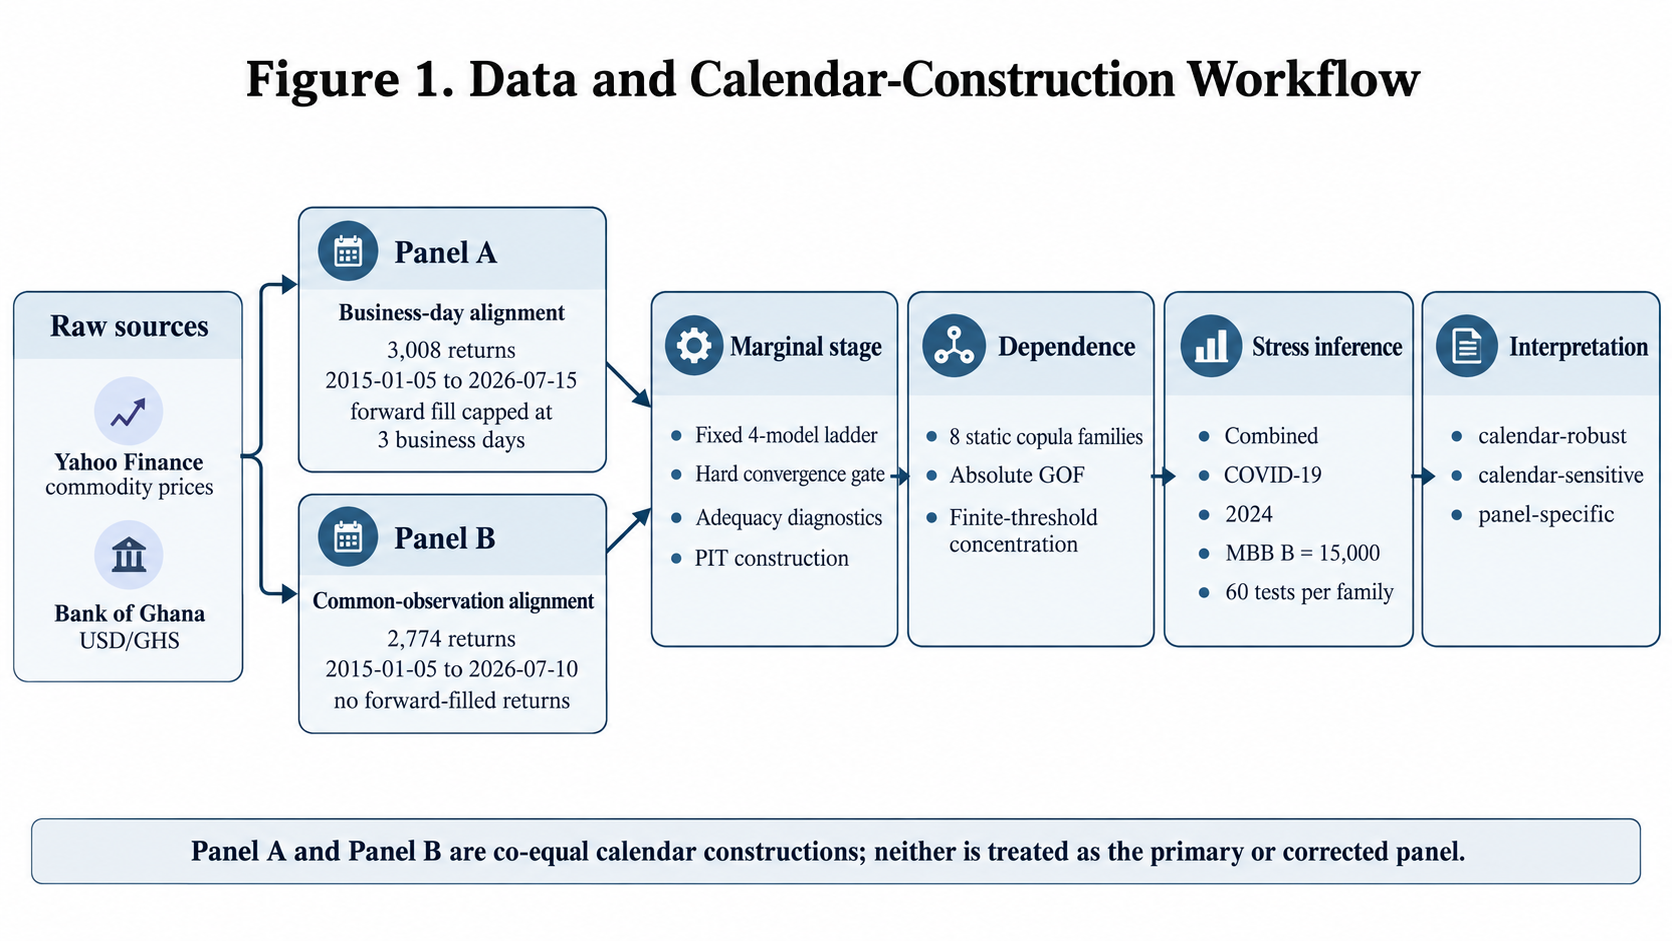
\includegraphics[width=\linewidth]{figures/publication/figure_01_calendar_workflow.png}
\caption{Data and calendar-construction workflow. Panel A uses business-day alignment with forward filling capped at three business days, whereas Panel B uses consecutive common actual-source observation dates without forward-filled returns. The two panels are treated as co-equal representations of the observation process.}
\label{fig:calendar-workflow}
\end{figure}

\subsection{Empirical finite-threshold tail-concentration profiles}
\label{sec:results-tailprofiles}

Figure~\ref{fig:tail-profiles} presents empirical lower- and upper-tail concentration measures at $q=0.025$, $0.05$, and $0.10$ for selected asset pairs under both calendar constructions. These quantities are finite-threshold empirical concentration measures and are not interpreted as asymptotic tail-dependence coefficients.

Across the selected pairs, concentration generally increases as the threshold widens from $q=0.025$ to $q=0.10$, although the magnitude and degree of agreement between Panels A and B vary across asset combinations. Cocoa--Gold displays broadly similar profiles under the two calendar constructions, particularly at the intermediate and wider thresholds. Cocoa--Brent shows clearer separation between the lower and upper tails, with lower-tail concentration exceeding upper-tail concentration throughout most of the threshold range in both panels.

Gold--WTI exhibits comparatively pronounced concentration in both tails, particularly at $q=0.10$. Although some panel-specific differences are present at the more extreme thresholds, both calendar constructions indicate substantial finite-threshold concentration for this pair as the threshold widens. Gold--Cedi, by comparison, displays lower concentration levels overall and somewhat greater differences between the two calendar constructions, particularly in the lower tail at the wider threshold.

The comparison therefore indicates that some empirical tail features are relatively stable to calendar construction whereas others are more sensitive to the treatment of nonsynchronous observations. This distinction motivates the subsequent absolute copula goodness-of-fit analysis rather than treating the empirical profiles alone as evidence of a particular parametric dependence structure.

\begin{figure}[htbp]
\centering
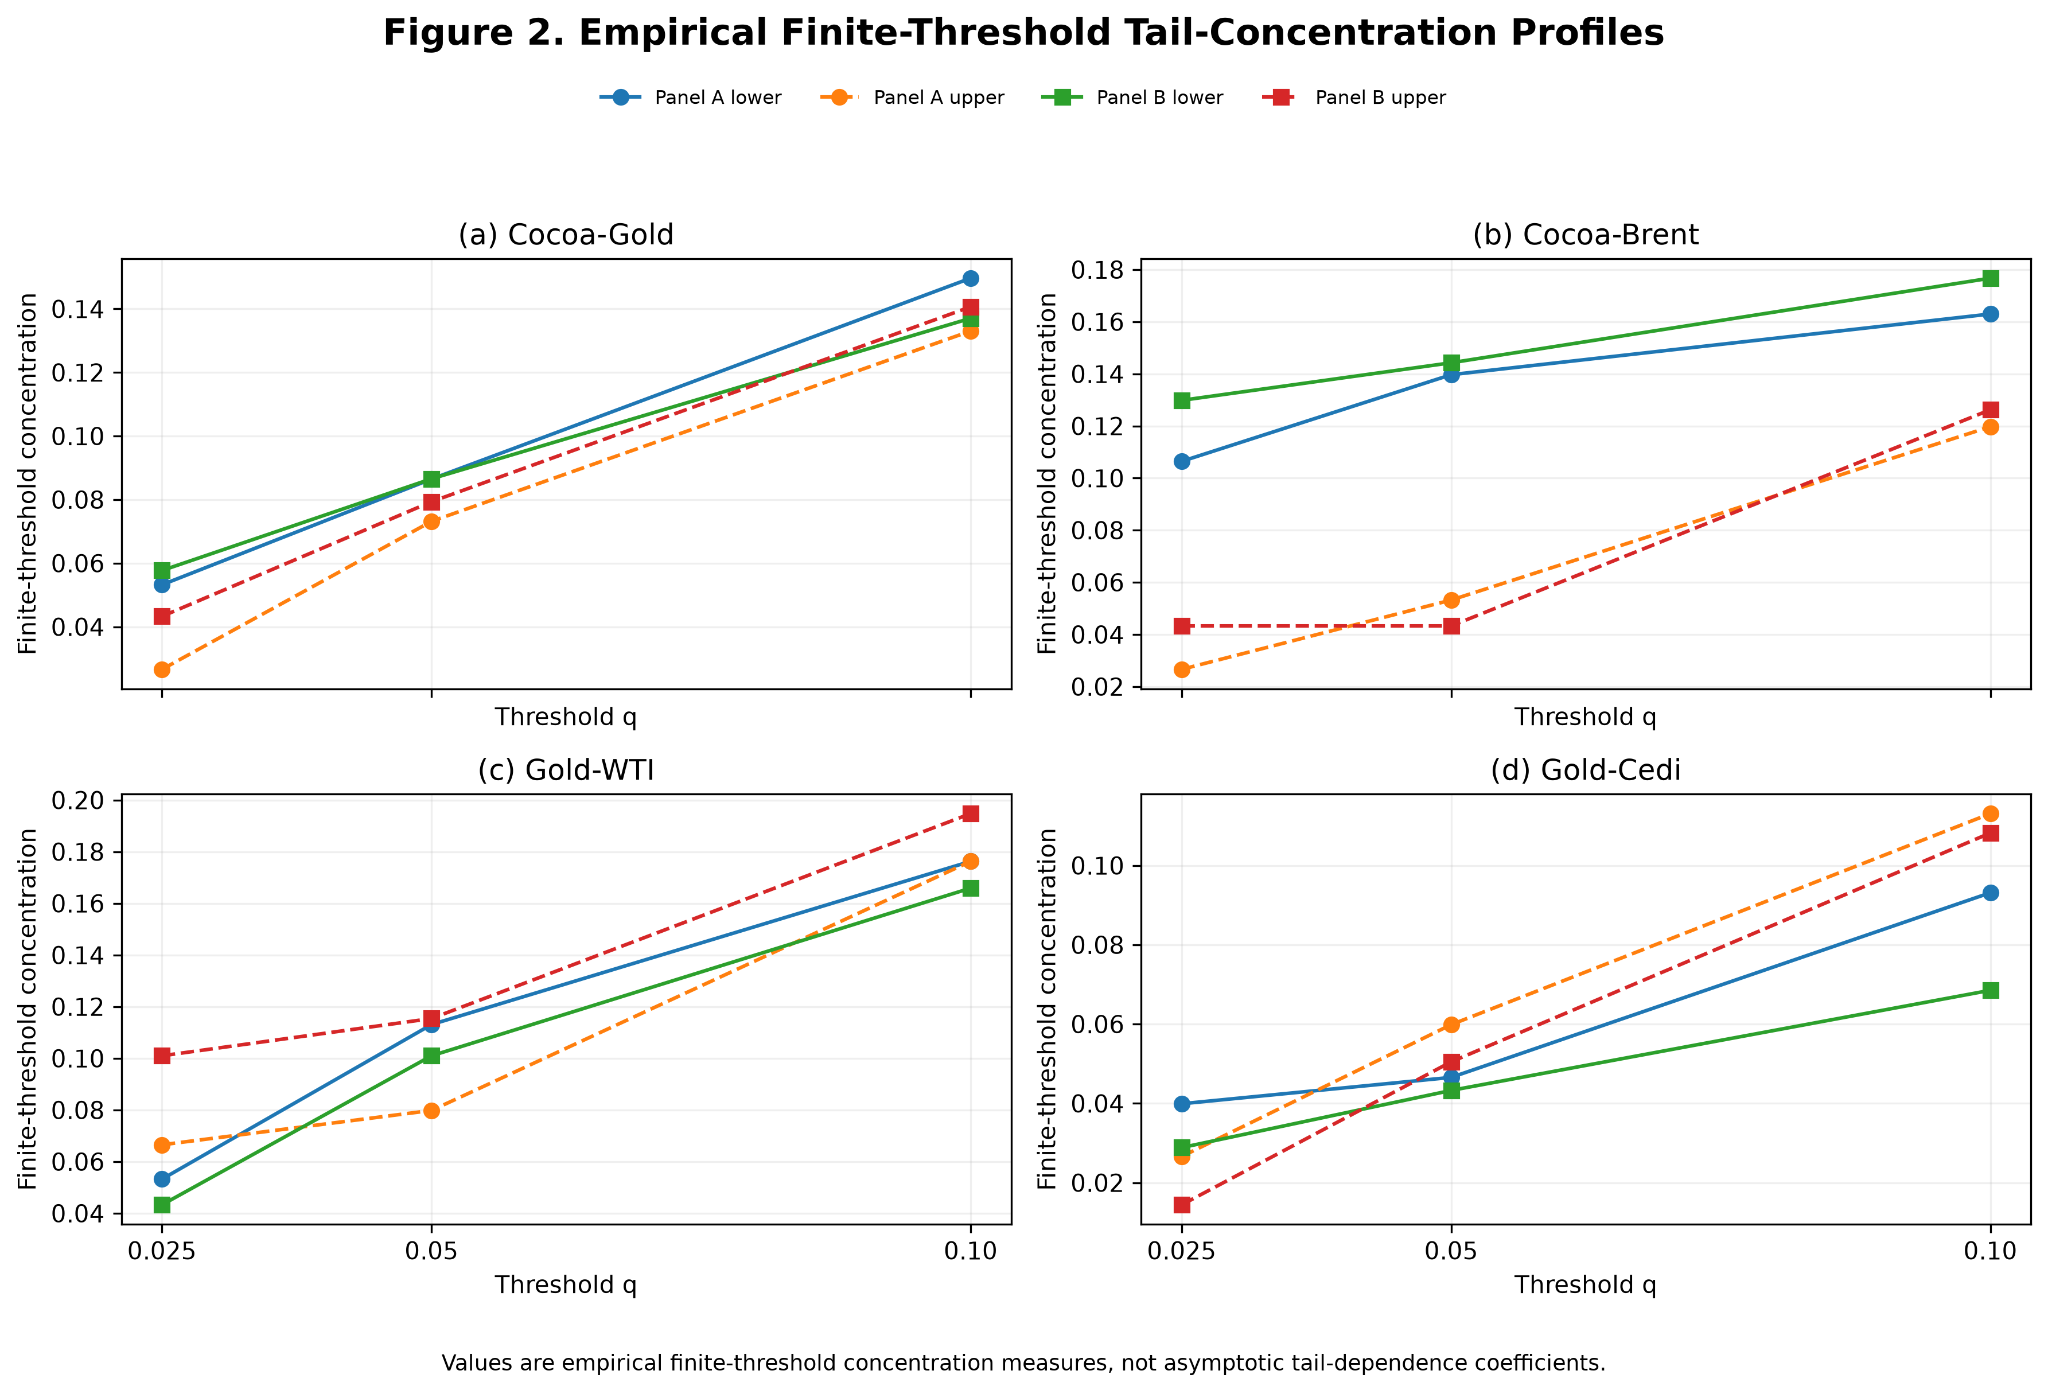
\includegraphics[width=\linewidth]{figures/publication/figure_02_tail_concentration_profiles.png}
\caption{Empirical finite-threshold tail-concentration profiles. Lower- and upper-tail empirical concentration at $q=0.025$, $0.05$, and $0.10$ for selected pairs under Panels A and B. The values are finite-threshold concentration measures and should not be interpreted as asymptotic tail-dependence coefficients.}
\label{fig:tail-profiles}
\end{figure}

\subsection{Static copula goodness-of-fit across calendar constructions}
\label{sec:results-gof}

Substantial differences emerge across asset pairs in the ability of the eight tested static copula families to pass the absolute goodness-of-fit assessment (Figure~\ref{fig:gof-heatmap}). Three commodity--commodity pairs---Gold--Brent, Gold--WTI, and Brent--WTI---produce a calendar-robust pattern of complete rejection. For each of these pairs, all eight tested static copula families are rejected in both Panel A and Panel B. The result therefore does not depend on the choice between the business-day and common-observation calendar constructions.

The four commodity--Cedi pairs show the opposite pattern. For Cocoa--Cedi, Gold--Cedi, Brent--Cedi, and WTI--Cedi, all eight tested families are non-rejected in both calendar constructions. This result is interpreted strictly as an absence of rejection under the applied goodness-of-fit tests; it does not establish that any particular copula family is the true dependence model.

The strongest calendar sensitivity occurs among the three Cocoa--commodity pairs. In Panel A, none of the eight families is non-rejected for Cocoa--Gold, Cocoa--Brent, or Cocoa--WTI, corresponding to complete eight-family rejection. In Panel B, however, six of eight families are non-rejected for Cocoa--Gold, while five of eight are non-rejected for both Cocoa--Brent and Cocoa--WTI. Thus, the absolute goodness-of-fit assessment for the Cocoa--commodity relationships depends materially on the observation-calendar construction.

The results therefore separate the asset pairs into three evidential categories: calendar-robust model inadequacy for Gold--Brent, Gold--WTI, and Brent--WTI; calendar-robust non-rejection for the four commodity--Cedi pairs; and calendar-sensitive adequacy for the three Cocoa--commodity pairs.

\begin{figure}[htbp]
\centering
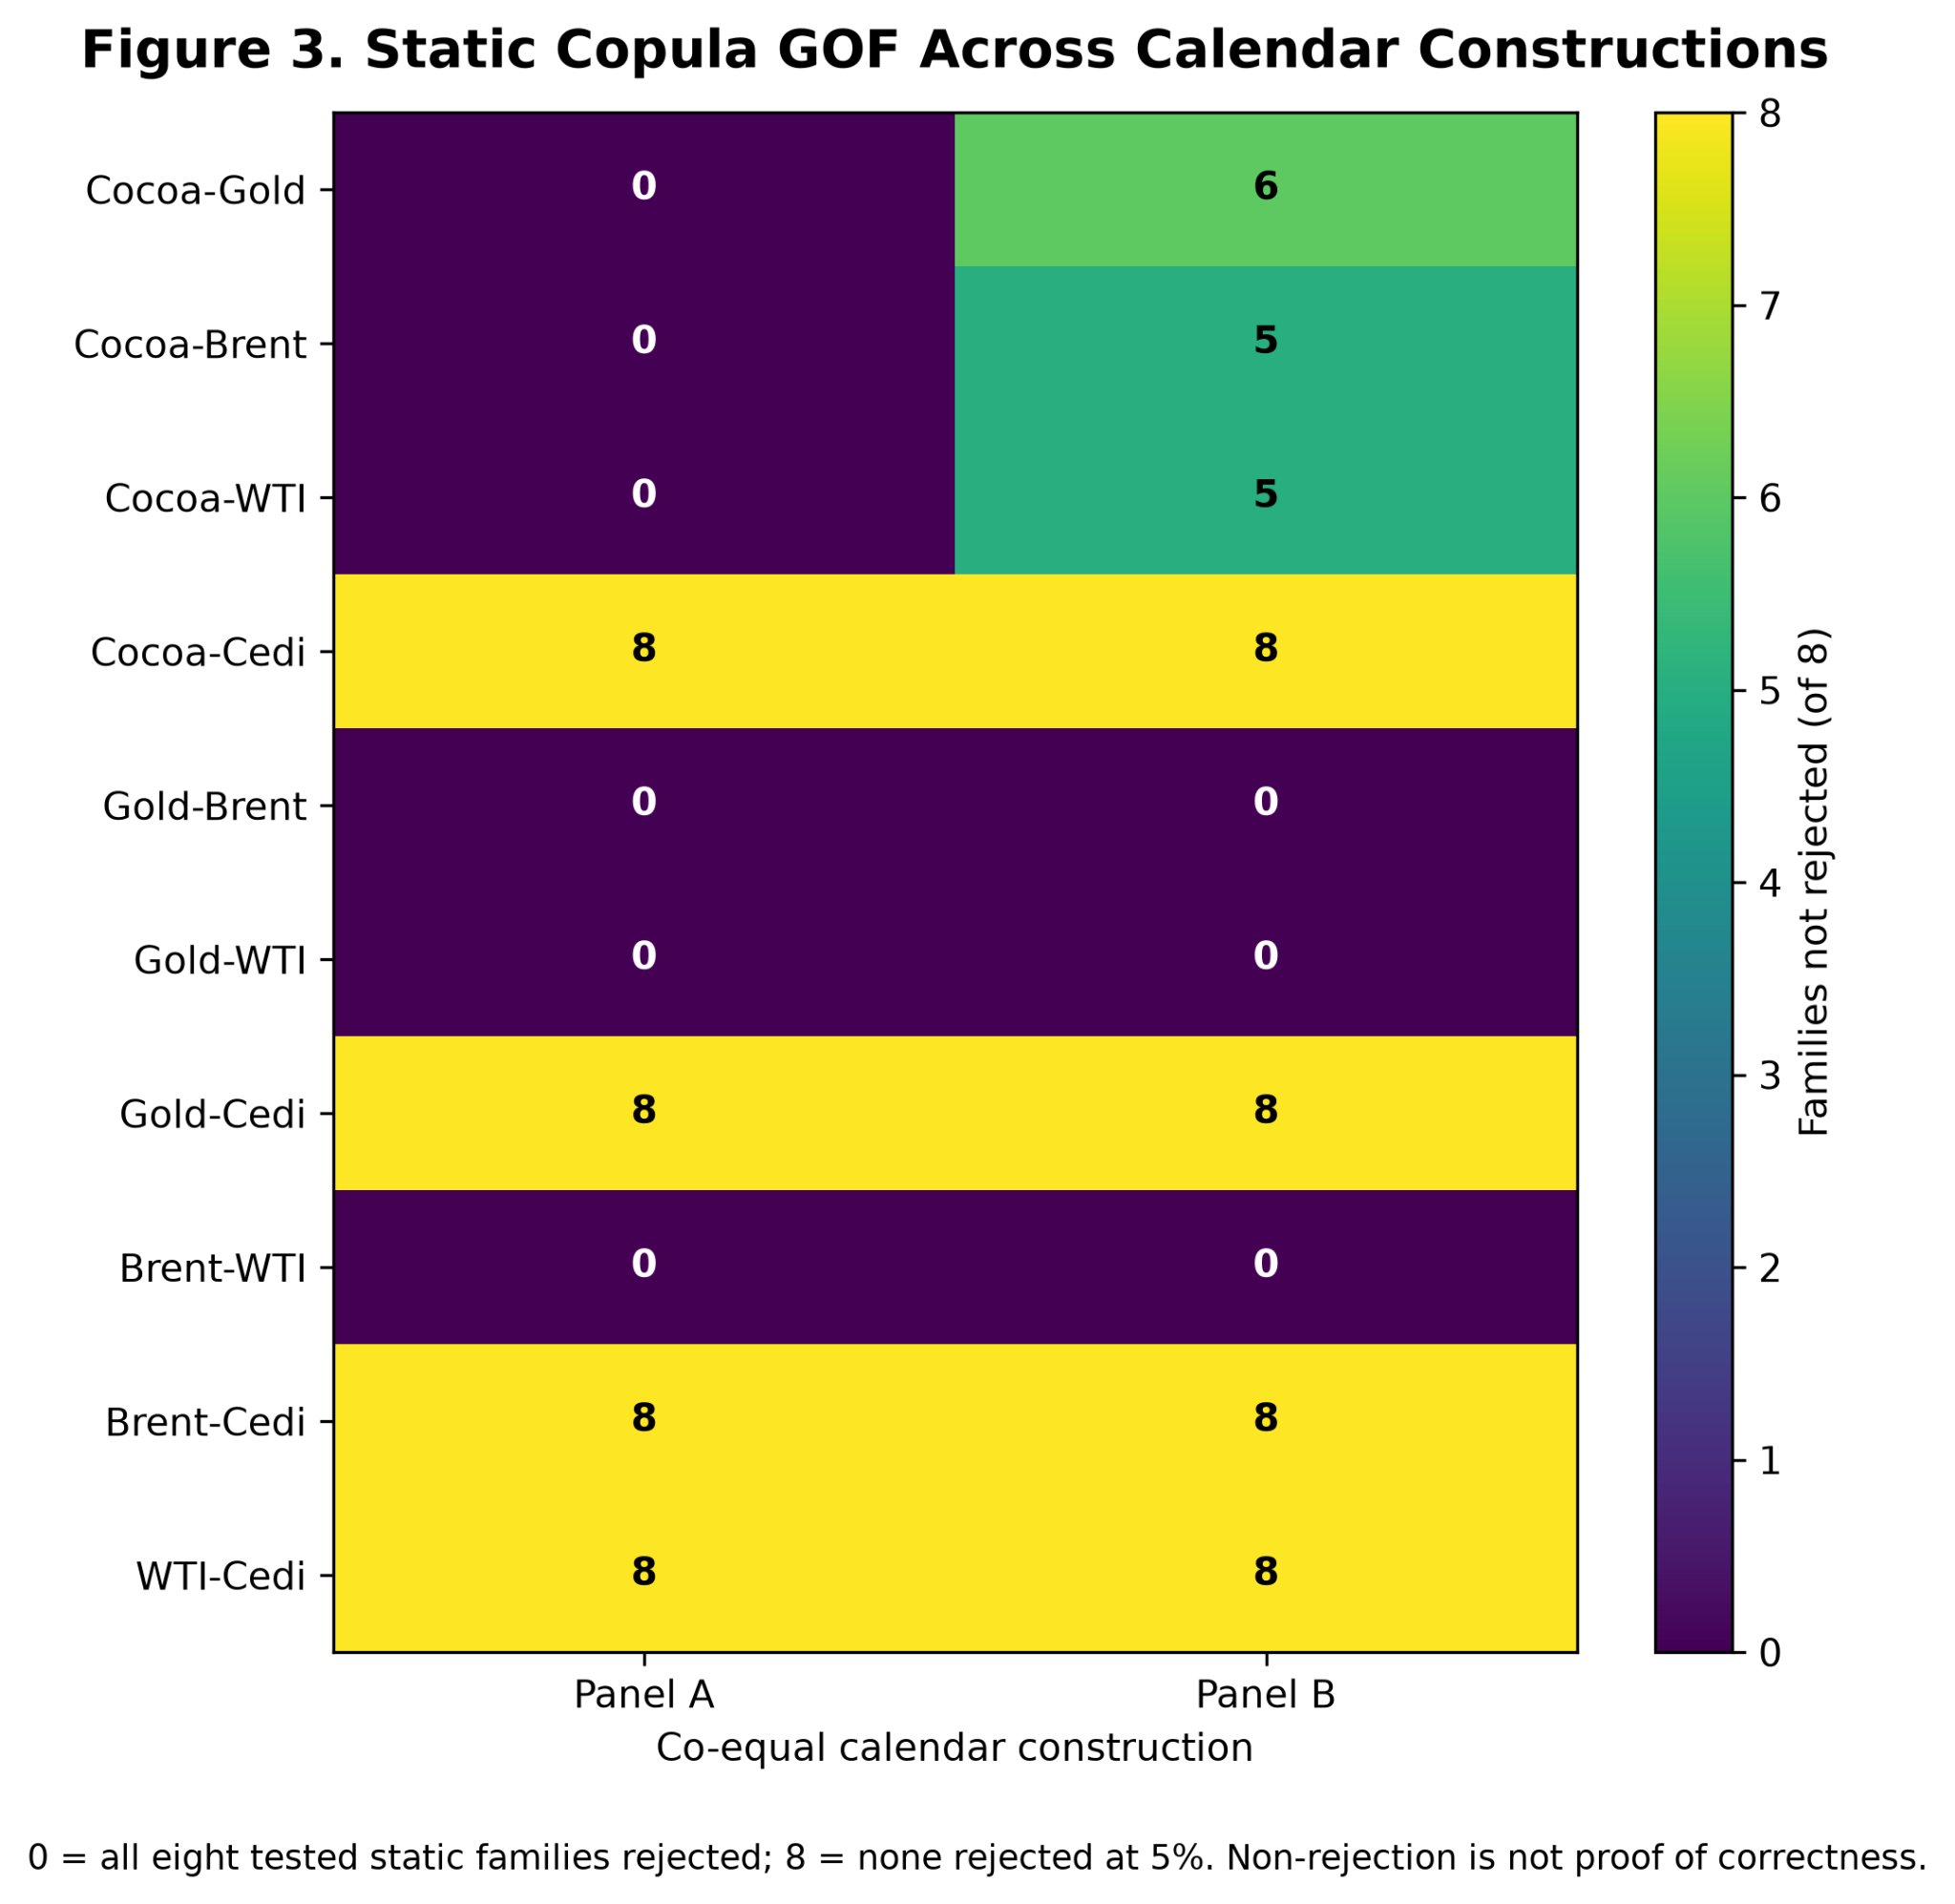
\includegraphics[width=0.82\linewidth]{figures/publication/figure_03_copula_gof_heatmap.png}
\caption{Static copula goodness-of-fit across calendar constructions. Each cell reports the number of the eight tested static copula families that were not rejected at the 5\% level. A value of zero indicates rejection of all eight tested families, whereas eight indicates that none was rejected. Non-rejection should not be interpreted as proof of model correctness.}
\label{fig:gof-heatmap}
\end{figure}

\subsection{Stress--calm tail-concentration inference}
\label{sec:results-calmstress}

Stress--calm comparisons were conducted separately for the combined stress definition, the COVID-19 period, and the 2024 stress period, with 60 tests undertaken within each panel--stress family. Figure~\ref{fig:stress-summary} distinguishes the nominal $p<0.05$ counts from the multiplicity-controlled results.

For the combined stress definition, 6 of 60 tests are nominally significant in Panel A and 5 of 60 in Panel B. The COVID-19 specification produces the largest number of nominal findings, with 13 of 60 tests in Panel A and 11 of 60 in Panel B. Under the 2024 specification, 6 of 60 tests are nominally significant in Panel A and 7 of 60 in Panel B.

These unadjusted counts do not translate into multiplicity-controlled discoveries. Across all three stress definitions and both calendar constructions, zero tests survive Bonferroni correction and zero survive Benjamini--Hochberg false-discovery-rate correction. Accordingly, the nominal $p<0.05$ findings are retained only as descriptive diagnostics and are not promoted to confirmatory evidence of stress-related changes in tail concentration.

The consistency of the adjusted result across the two calendar constructions is particularly important. Although the number and identity of nominal findings vary to some extent between Panels A and B, the inferential conclusion after multiplicity control is invariant: the analysis does not identify a stress--calm tail-concentration difference that meets the prespecified multiplicity-controlled evidential threshold.

\begin{figure}[htbp]
\centering
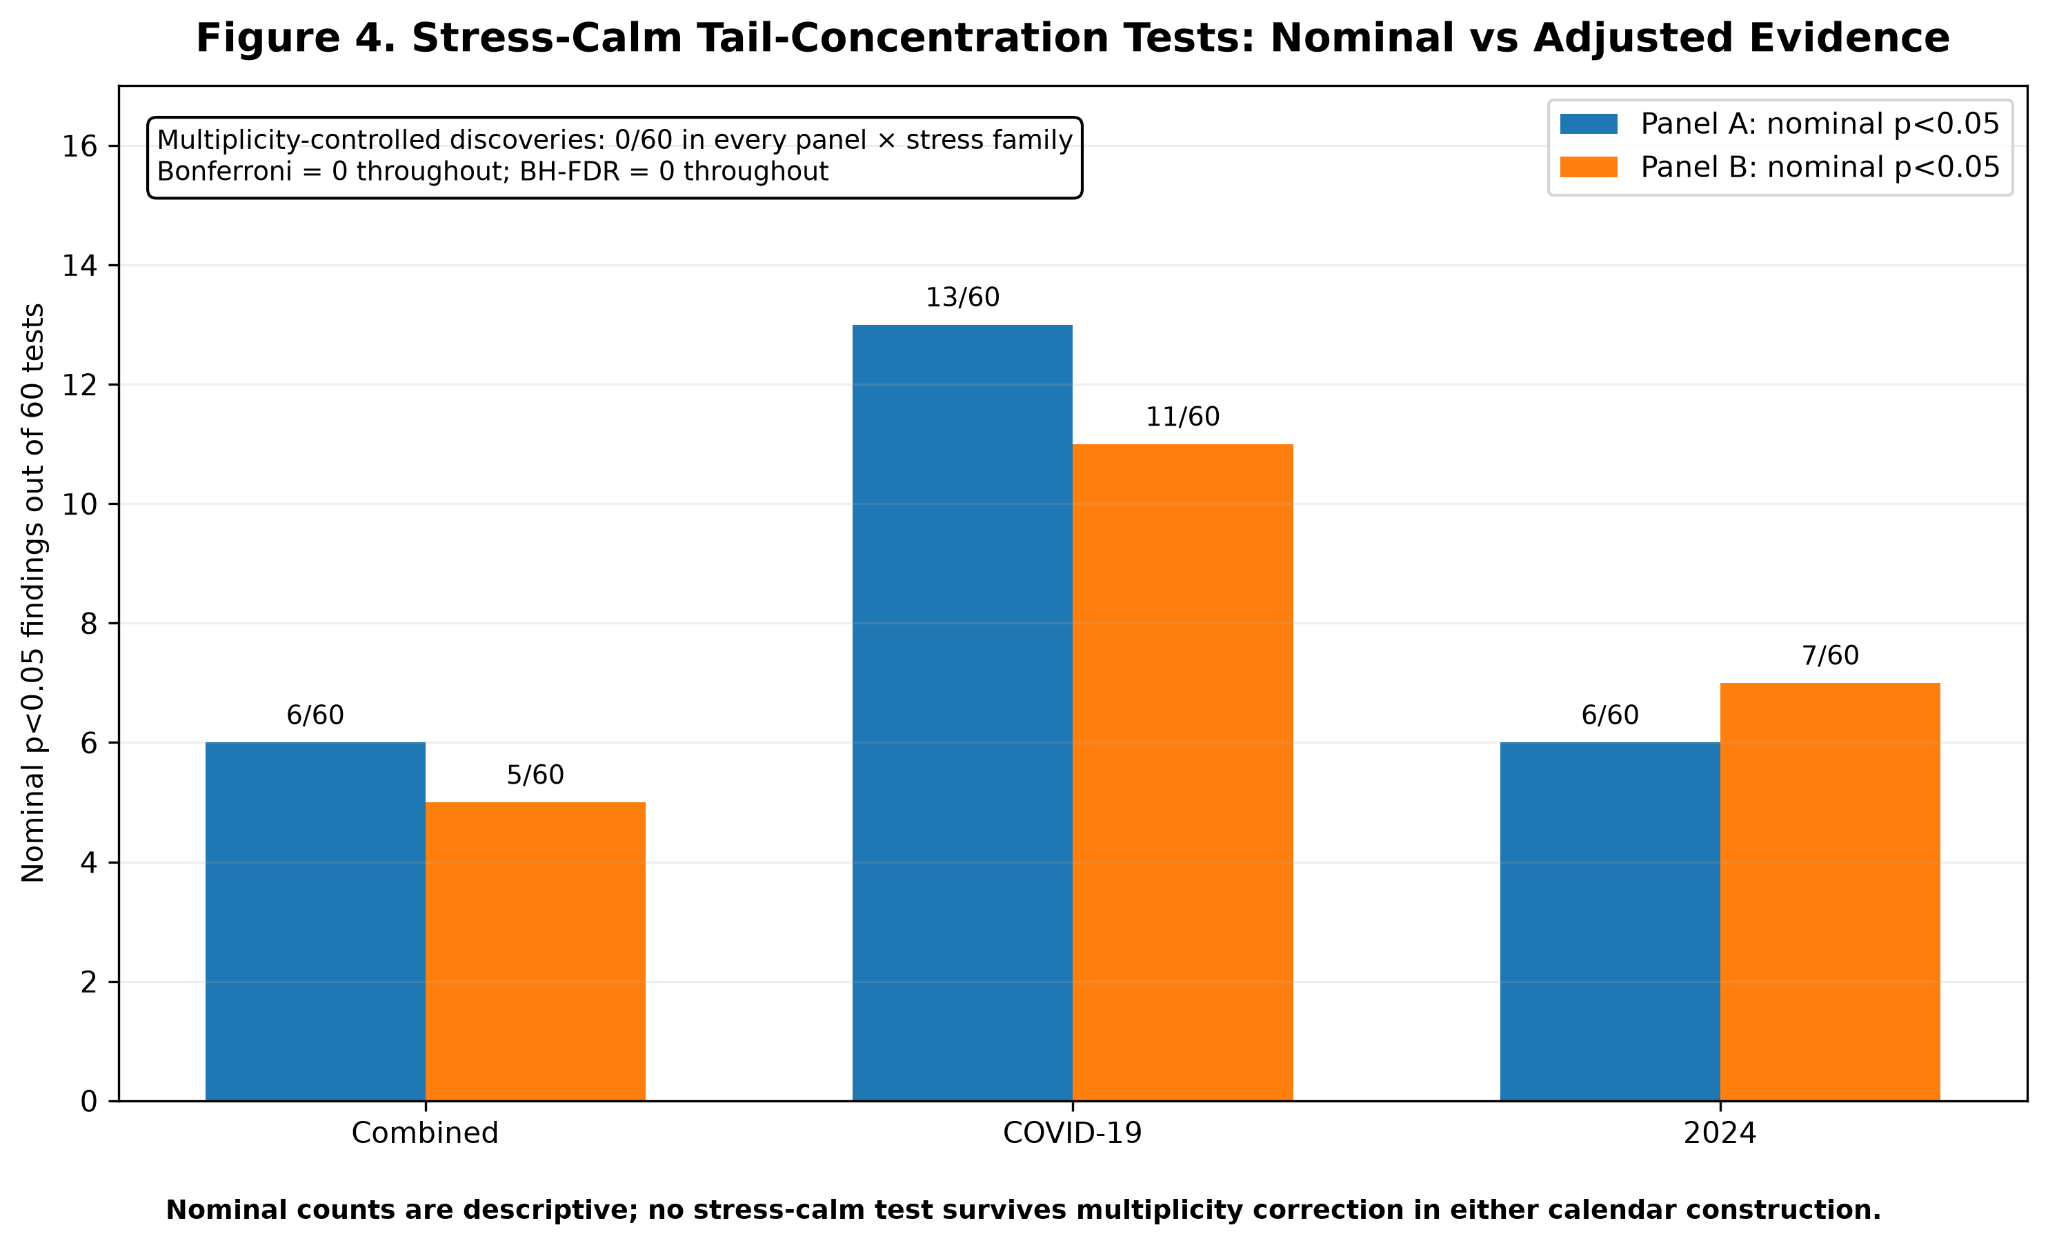
\includegraphics[width=\linewidth]{figures/publication/figure_04_stress_summary.png}
\caption{Stress--calm tail-concentration tests: nominal versus adjusted evidence. Bars show the number of nominal $p<0.05$ findings among 60 tests for each stress definition. None of the tests survives either Bonferroni or Benjamini--Hochberg correction in either calendar construction.}
\label{fig:stress-summary}
\end{figure}

\subsection{Cedi-related diagnostics and sensitivity analyses}
\label{sec:results-cedi}

Additional analyses were undertaken because the selected Cedi marginal reference model did not satisfy the marginal adequacy requirement in either calendar construction. The Cedi-related dependence and extreme-value results are therefore interpreted conditionally on this limitation rather than being treated as unrestricted model-based evidence.

The Panel B peaks-over-threshold analysis shows sensitivity in the estimated generalized Pareto shape parameter, 99\% Value-at-Risk, and 99\% Expected Shortfall as the threshold quantile varies (Supplementary Figure~\ref{fig:s1-evt}). The $q=0.90$ specification is retained as a reference point in the sensitivity display, but the resulting EVT quantities remain conditional diagnostics because of the unresolved Cedi marginal inadequacy.

The Panel A A--G sensitivity exercise likewise demonstrates that nominal findings vary with the treatment applied to the Cedi series (Supplementary Figure~\ref{fig:s2-ag}). The number of nominal $p<0.05$ findings across the seven treatments is 3, 3, 2, 0, 2, 2, and 2, respectively. In particular, treatment D produces no nominal findings. For the illustrated Brent--Cedi lower-tail comparison at $q=0.05$, several alternative treatments yield unadjusted $p$-values below 0.05, whereas treatment D yields $p=0.641$. These results reinforce the sensitivity of unadjusted Cedi-related findings to data treatment and support their classification as diagnostics rather than headline discoveries.

The separate PIT-clipping audit provides evidence that the observed numerical clipping artifact is negligible for the prespecified tail analysis (Supplementary Figure~\ref{fig:s3-pit}). Three Cedi observations are tied at the clipping boundary of $10^{-6}$. Recovering their residual ordering alters only two pseudo-observations, does not change membership of the $q=0.025$, $0.05$, or $0.10$ tail sets, and produces a maximum absolute change in the observed goodness-of-fit statistic of approximately $0.000262$. Thus, although the clipping artifact is explicitly investigated, it does not account for the substantive cross-panel results reported above.

\subsection{Cross-panel synthesis of the evidence}
\label{sec:results-synthesis}

Table~\ref{tab:crosspanel} summarizes the findings that are robust and those that are sensitive to calendar construction. Several results are stable across both panels. All four commodity--Cedi pairs have all eight tested static copula families non-rejected under both calendar constructions. Conversely, Gold--Brent, Gold--WTI, and Brent--WTI show complete eight-family rejection in both panels. Most importantly for the stress analysis, neither panel produces any Bonferroni- or BH-FDR-adjusted stress--calm discovery under the combined, COVID-19, or 2024 stress definitions.

The principal calendar-sensitive findings concern Cocoa's dependence with the other commodities. Cocoa--Gold, Cocoa--Brent, and Cocoa--WTI produce complete rejection of all eight static copula families under Panel A, whereas Panel B retains six, five, and five non-rejected families, respectively. These results show that the inferred adequacy of conventional static copulas for the Cocoa--commodity relationships is sensitive to the treatment of nonsynchronous trading calendars.

Taken together, the results support three evidential classifications used throughout the remainder of the study: \emph{calendar-robust findings}, for which the substantive result is preserved under both calendar constructions; \emph{calendar-sensitive findings}, for which the inference changes with the observation-calendar treatment; and \emph{panel-specific diagnostics}, which are informative within one construction but are not promoted to cross-panel conclusions.

The strongest cross-panel conclusions are therefore not based on the number of nominal findings alone, but on the combination of absolute model adequacy, robustness to calendar construction, and multiplicity-controlled inference.

\begin{table}[htbp]
\centering
\caption{Cross-panel evidence summary.}
\label{tab:crosspanel}
\small
\begin{tabular}{p{0.22\linewidth}p{0.34\linewidth}p{0.34\linewidth}}
\toprule
Feature & Panel A: business-day alignment & Panel B: common-observation alignment \\
\midrule
Return observations & 3,008 & 2,774 \\
Return period & 2015-01-05 to 2026-07-15 & 2015-01-05 to 2026-07-10 \\
Alignment rule & Business-day; forward fill $\leq 3$ business days & Consecutive common actual-source dates \\
Commodity--Cedi GOF & All 4 pairs: 8/8 not rejected & All 4 pairs: 8/8 not rejected \\
Robust 0/8 not rejected & Gold--Brent; Gold--WTI; Brent--WTI & Gold--Brent; Gold--WTI; Brent--WTI \\
Cocoa commodity pairs & 0/8 not rejected for all 3 pairs & 6/8, 5/8, 5/8 not rejected \\
Corrected stress discoveries & 0 under all 3 families & 0 under all 3 families \\
Role & Co-equal panel & Co-equal panel \\
\bottomrule
\end{tabular}
\end{table}

% Supplementary diagnostic figures. These can be moved to a separate
% supplement file when the target journal's submission format is fixed.
\begin{figure}[htbp]
\centering
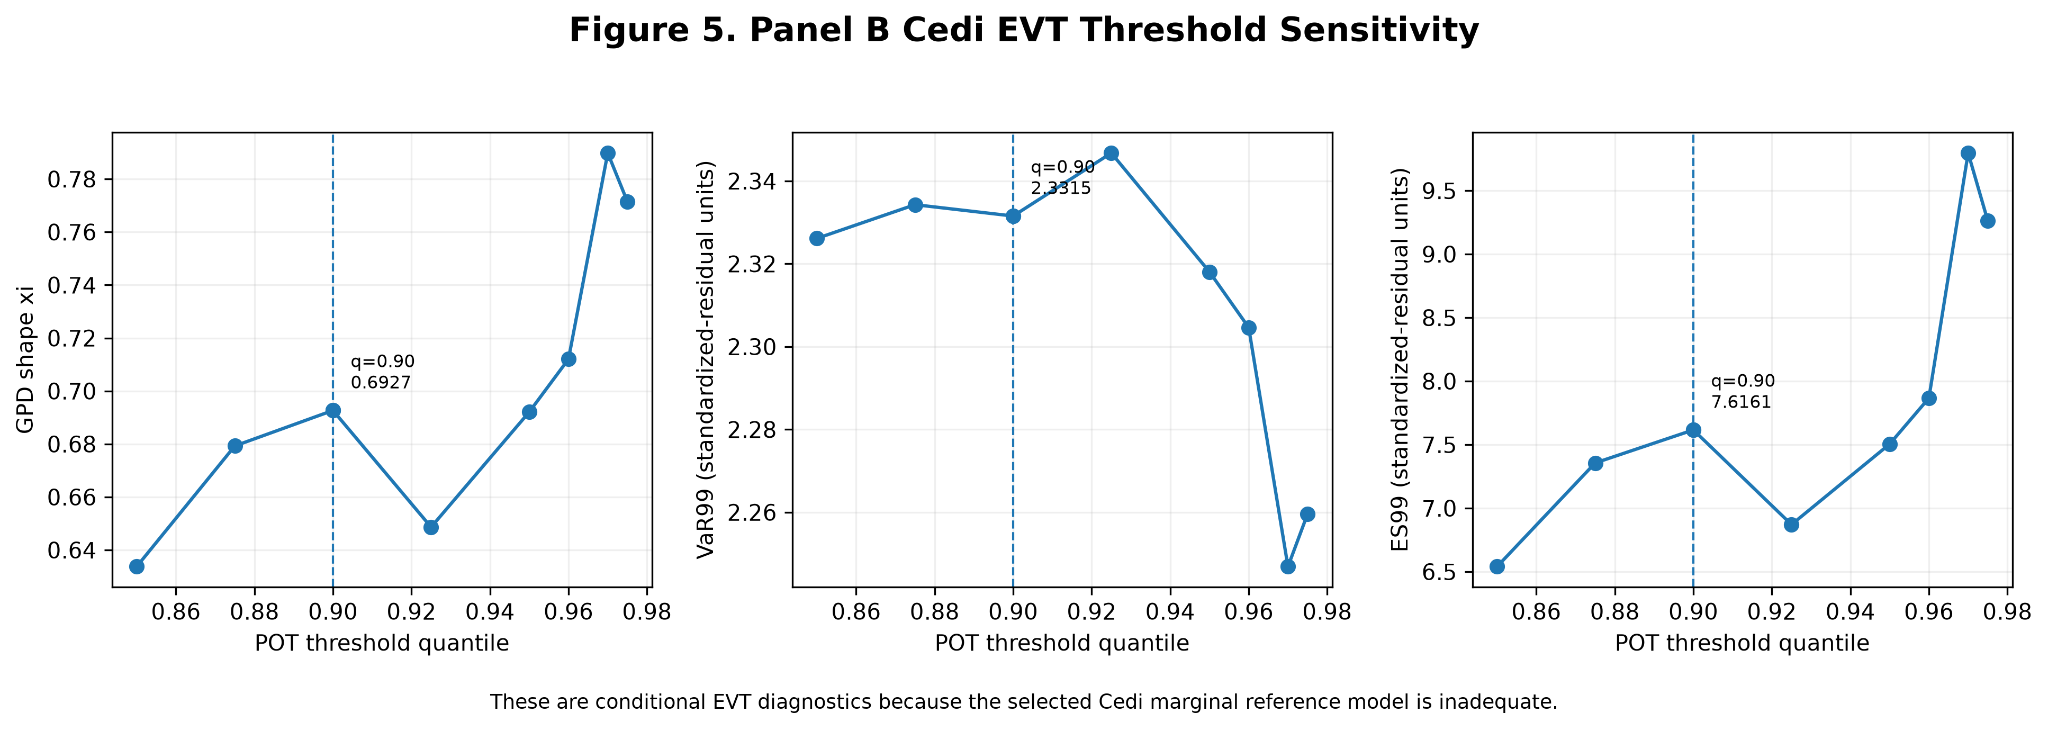
\includegraphics[width=\linewidth]{figures/publication/figure_S1_cedi_evt_threshold_sensitivity.png}
\caption{Panel B Cedi EVT threshold sensitivity. These are conditional diagnostics because the selected Cedi marginal reference model is inadequate.}
\label{fig:s1-evt}
\end{figure}

\begin{figure}[htbp]
\centering
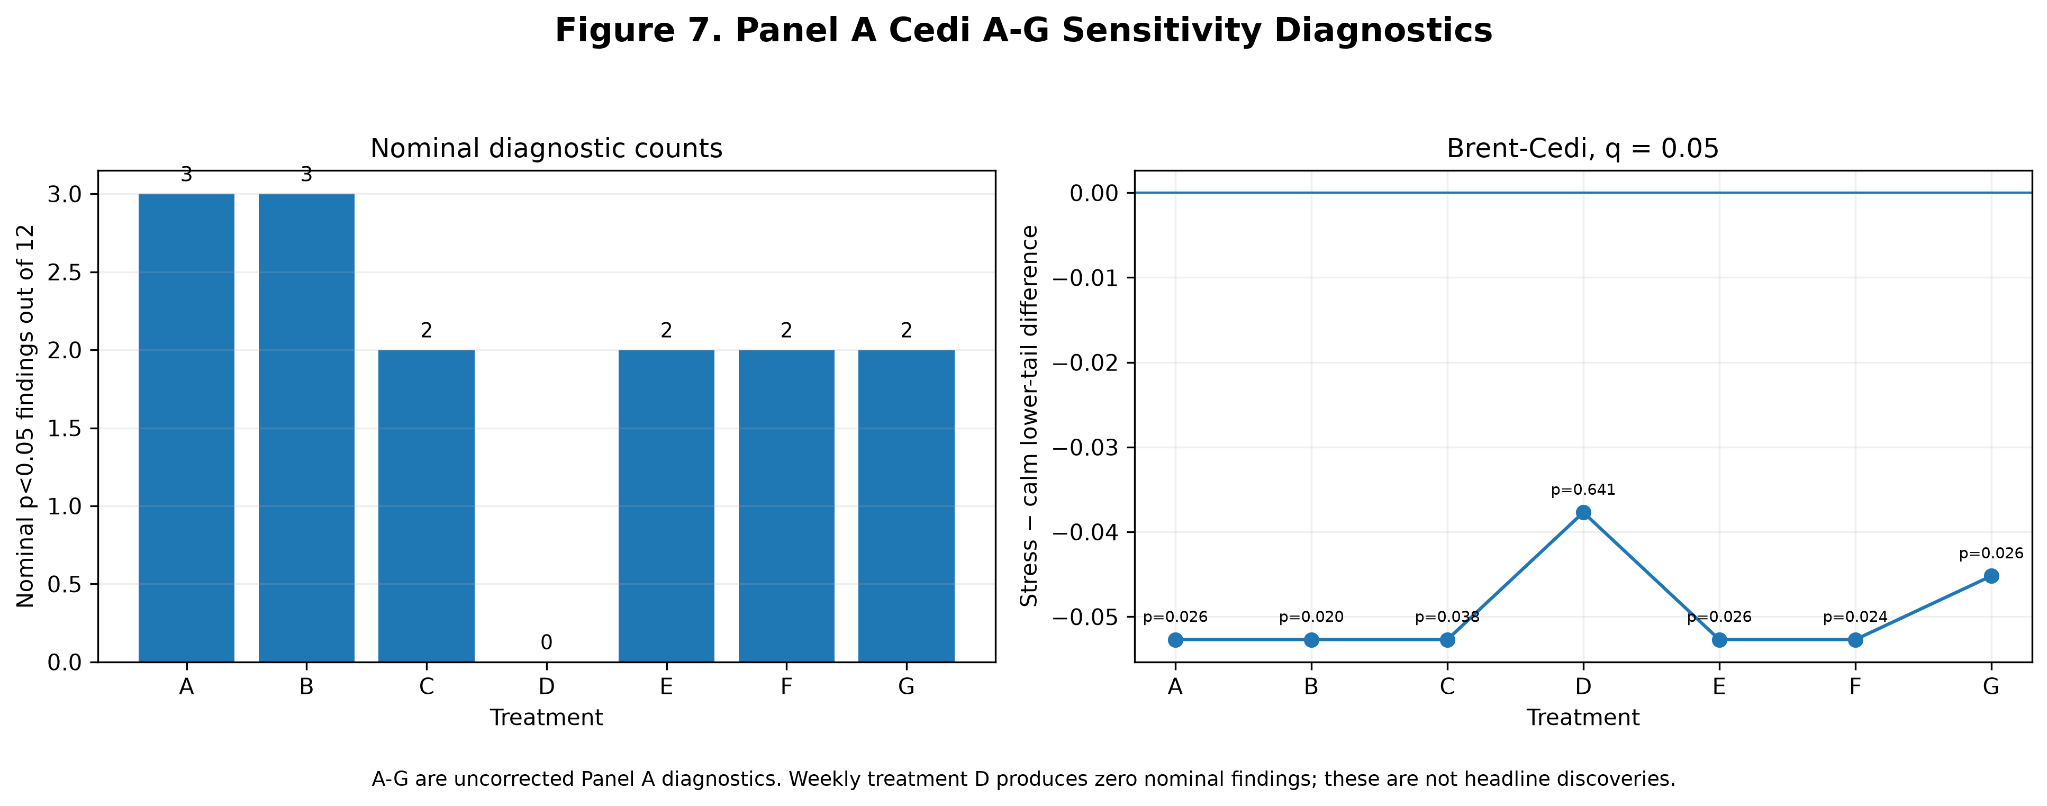
\includegraphics[width=\linewidth]{figures/publication/figure_S2_cedi_AG_sensitivity.png}
\caption{Panel A Cedi A--G sensitivity diagnostics. The displayed counts and $p$-values are uncorrected diagnostics and are not treated as headline discoveries.}
\label{fig:s2-ag}
\end{figure}

\begin{figure}[htbp]
\centering
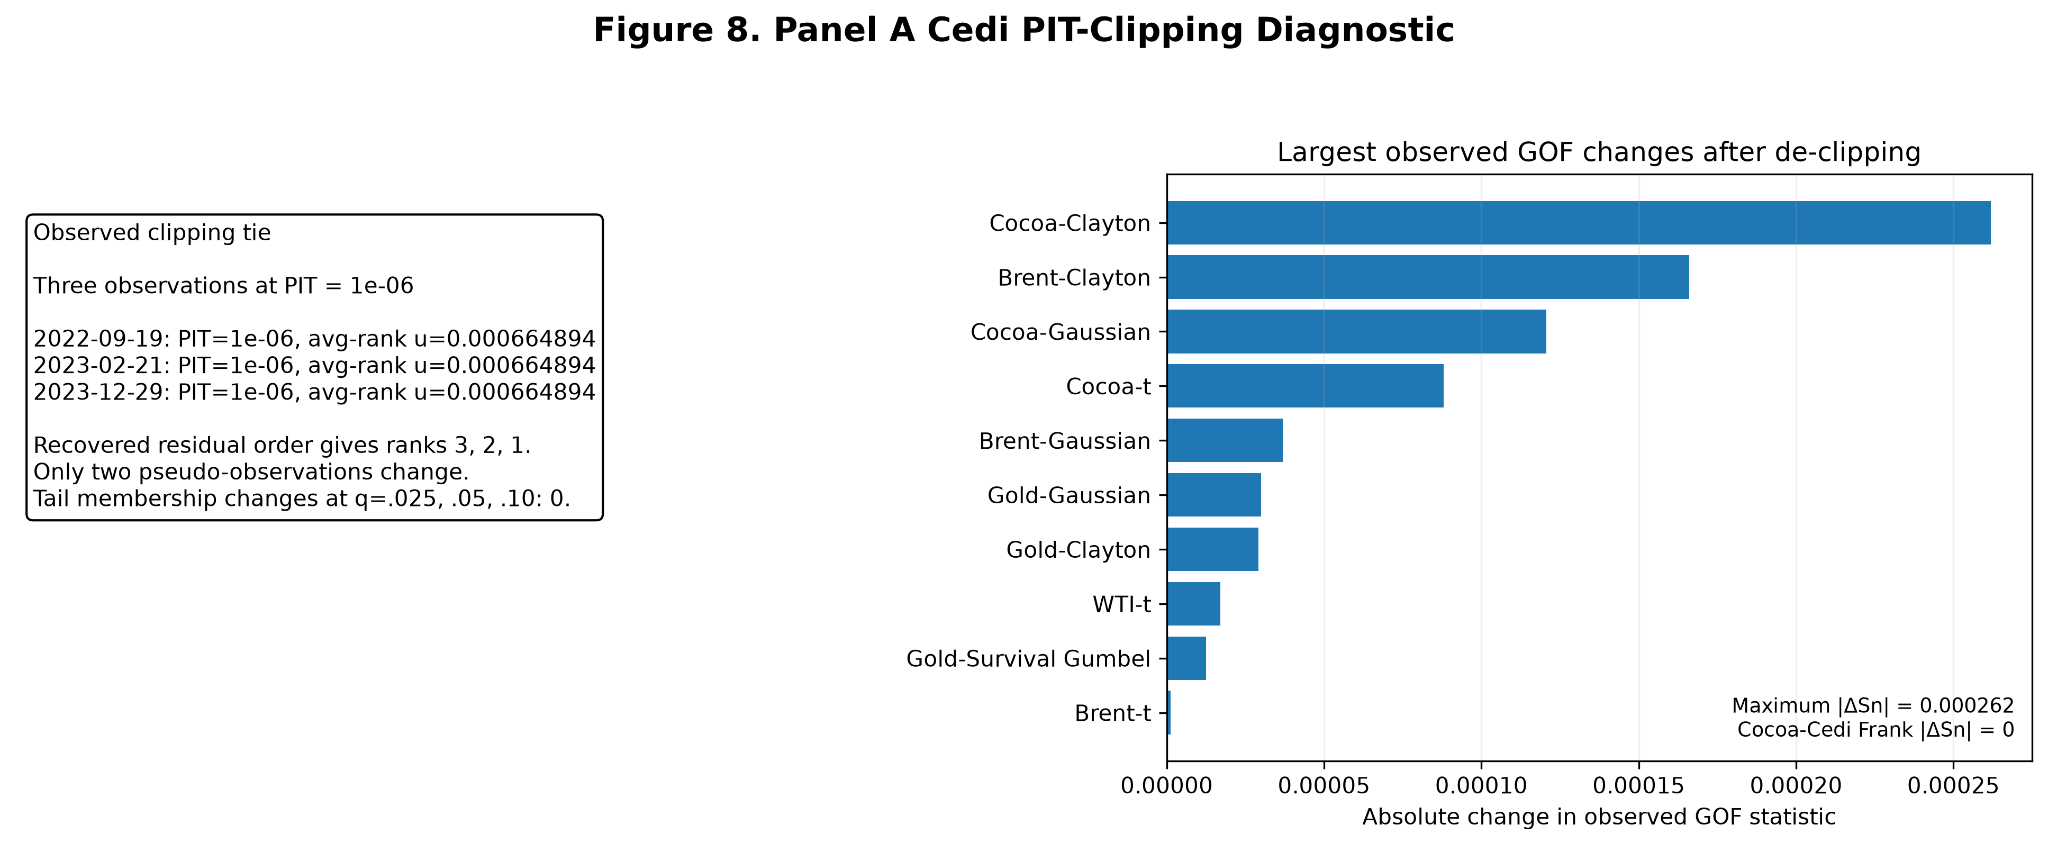
\includegraphics[width=\linewidth]{figures/publication/figure_S3_pit_clipping_diagnostic.png}
\caption{Panel A Cedi PIT-clipping diagnostic. The observed clipping tie has negligible numerical consequences for the prespecified tail sets and copula goodness-of-fit statistics.}
\label{fig:s3-pit}
\end{figure}
